
%Whereas during training, we allow users to fail at task completion for improved learning, during assistance in tasks, such as activities of daily living (ADL), we may want to insist on task success, user safety, or both. In these situations, we can modify the proposed filter to actively provide assistance. Instead of using a null controller input as the alternative to user input, we can engage the controller and replace rejected actions with optimal control, calculated by an MPC. In the next two subsections, we provide simulation results that demonstrate system behavior when the MIG-based filter is employed in assistance mode.

When assisting users in physical tasks, there are two highly desired features of a shared control paradigm. For one, we may want to insist on task success, user safety, or both even for unskilled users. Secondly, it should remain as transparent as possible to users at times when they do not require assistance at the task. In the simulation results presented below, we show that the proposed filter-based shared control paradigm in assistance mode possesses both features---it can successfully assist in task completion and/or keep a simulated user safe, while remaining sensitive to the user's skill level and engaging minimally. 

%
%\section{MIG criterion}
%
%Descent proofs. XXX
%
%	\begin{prop}\label{prop:: descent}
%	Consider systems with state $x$ and control $u$ and an objective given by \eqref{eq:: cost_wo_u}. Then, the control policy given by \eqref{eq:: u_alphad} is a descent direction for all $t\in[t_o, t_f]$. Further, if there exists $t\in[t_o, t_f]$ for which the MIG is negative, then the feedback policy in \eqref{eq:: u_alphad} will decrease the cost. Moreover, this feedback policy converges to the local minimizer trajectory, as stated in Definition 1. 
%	\end{prop}
%	\begin{proof}
%	Using a first-order Taylor expansion, we write
%	\begin{equation}\label{eq:: Te1}
%	J_1(v(t) + w(t)) \approx J_1(v(t)) + \frac{\partial J_1}{\partial u(t)}\Big\rvert_{v(t)}\cdot w(t). 
%	\end{equation}
%	For objectives of the form in \eqref{eq:: cost_wo_u}, we use the G\^ateaux derivative to calculate the gradient of the cost with respect to the control 
%	\begin{align}\label{eq:: Te}
%	\frac{d}{d\epsilon}J_1(v(t) + \epsilon w(t))\Big\rvert_{\epsilon=0} =& \int_{t_o}^{t_f} \rho(t)^TB(t)\cdot w(t)\,\mathrm{d}t.\end{align}
%	From \eqref{eq:: Te1} and \eqref{eq:: Te}, the first-order change in cost can be approximated with 
%	\begin{align*}
%	\Delta J_1 \approx \int_{t_o}^{t_f} \rho^T(t) B(t) \cdot w(t) \mathrm{d}t.
%	\end{align*}
%	Equivalently, using \eqref{eq:: MIG_noU}, we can write
%	\begin{align*}
%	\Delta J_1 \approx \int_{t_o}^{t_f} \frac{dJ_1}{d\lambda_+} \mathrm{d}t, 
%	\end{align*}
%	which, with the update of \eqref{eq:: u_alphad} and given that $\alpha_d < 0 $, becomes
%	\begin{align*}
%	\Delta J_1 \approx \int_{t_o}^{t_f} \alpha_d \lVert\rho^T(t) B(t)\rVert_{(\Lambda(t)+R)^{-1}}^2 \mathrm{d}t \le 0.
%	\end{align*}
%
%	We examine the case of the equality, such that 
%	\begin{align*}
%	\Delta J_1 = 0 &\Leftrightarrow \rho^T(t) B(t) = 0~\forall~t\in[t_o, t_f]\\
%	&\Leftrightarrow \frac{dJ_1}{d\lambda_+} = 0~\forall~t\in[t_o, t_f].
%	\end{align*}
%	If there exists $t\in[t_o,t_f]$ for which $dJ_1/d\lambda_+ < 0$, then $\Delta J_1 <0$. 
%	The change in cost, to first order, will be zero if and only if $\rho^T(t) B(t) = 0$ for all $t \in [t_o, t_f]$, which is the condition for a minimum according to Pontryagin's Maximum Principle (for objectives of the form in \eqref{eq:: cost_wo_u}).
%	\end{proof}
%   
%    Next, we prove that one can scale the descent direction in an arbitrary way, differently across the time-horizon, and still obtain a descent direction, provided that the direction of the update is maintained. 
%    
%    \begin{figure}[h]
%	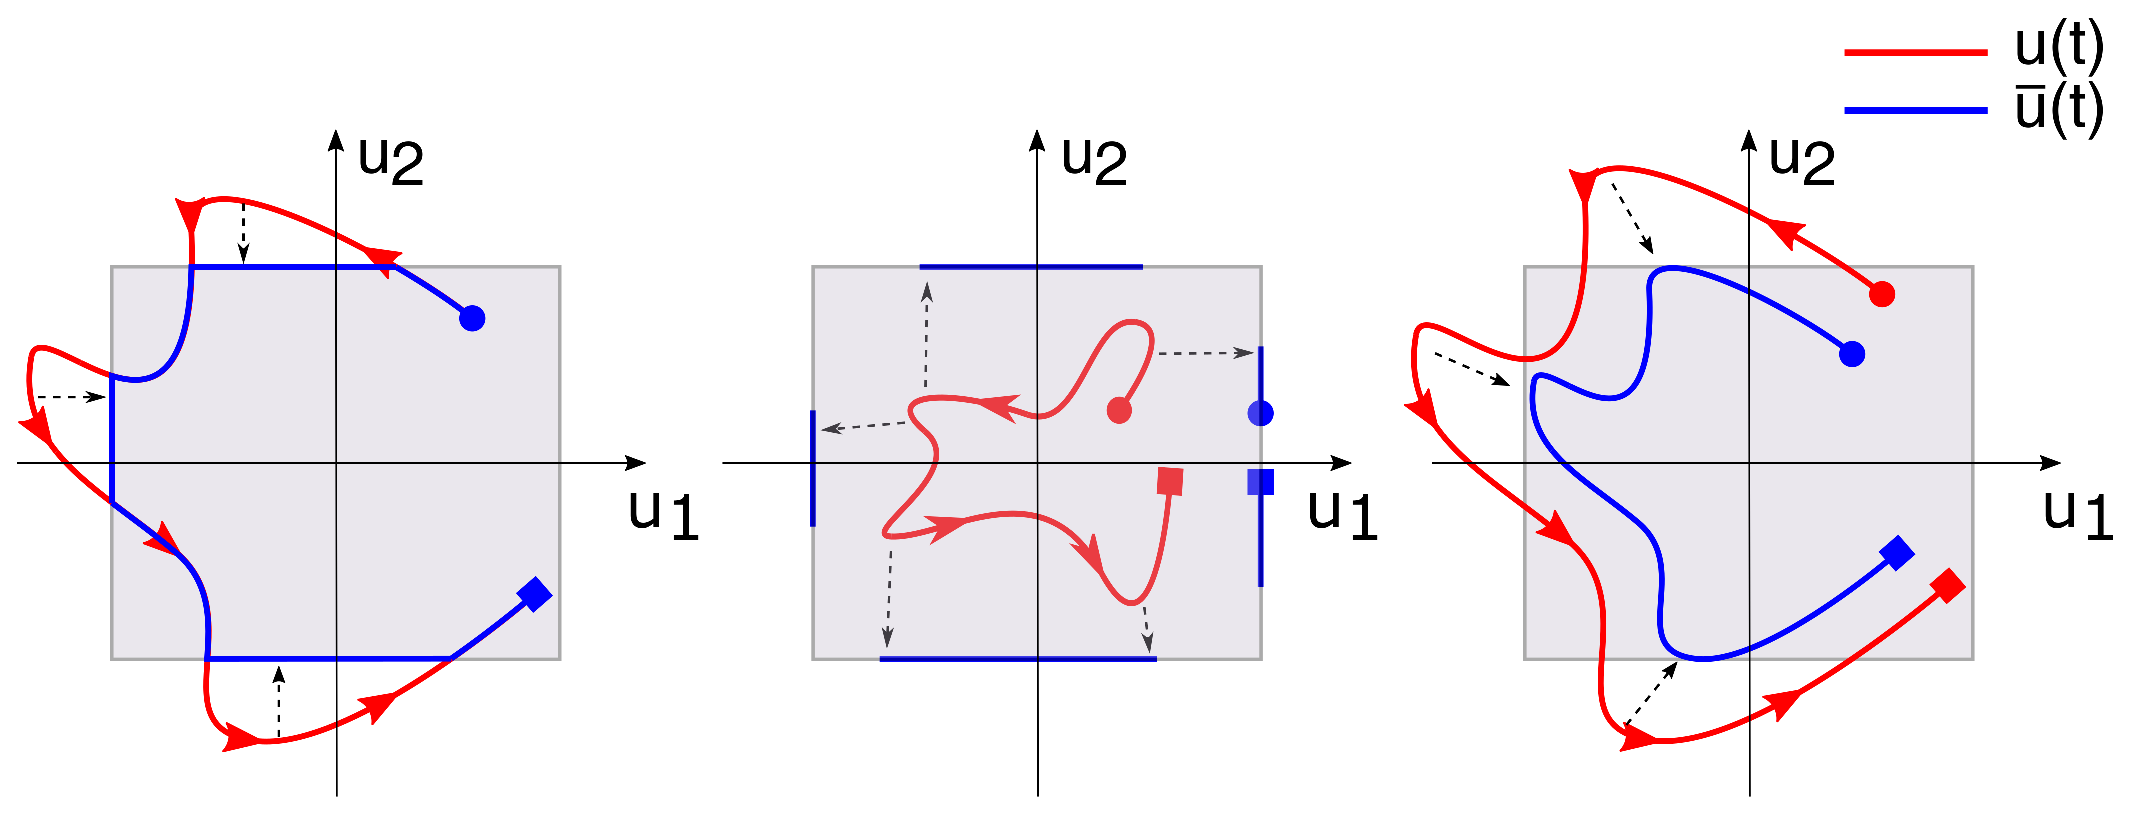
\includegraphics[width=\linewidth, keepaspectratio]{Scaling.eps}
%    \caption{Cases of control scaling that remain valid descent directions for the proposed needle-variation controller. The left figure shows control clipping, where values are saturated at a specific threshold; the middle figure shows arbitrary stretching to the saturation limits; the right figure shows proportional scaling that maintains the same direction of the applied control. Control curves are a function of time and arbitrarily shown for a 2-input system for easier visualization. Simulation results in this paper use control clipping.}
%    \label{fig: Descent Direction}
%    \end{figure}    
%    
%	\begin{prop}\label{prop:: saturated_descent_noad}
%	Consider systems with state $x$ and control $u$ and an objective metric given by \eqref{eq:: cost_wo_u}. Let $\Gamma(t) \succ 0$ be a diagonal matrix. The control update $w(t)$ given by \eqref{eq:: u_alphad} remains a descent direction for the entire trajectory even when scaled to $w_s(t) = \Gamma(t) w(t)$.
%	\end{prop}
%	\begin{proof}
%	Consider the update policy in \eqref{eq:: u_alphad} with scaled control $\bar{u}(t)$. Let $w_s(t)$ indicate the perturbation after scaling, such that $\bar{u}(t) = v(t) + w_s(t)$, where $w_s(t) = \Gamma(t) w(t)$, where the diagonal elements of $\Gamma(t)$, $\gamma_i(t) \ge 0$, can be different from each other.
%	
%	From Proposition \ref{prop:: descent_noad}, the cost change, approximated to first-order, is then
%	\begin{align}\label{eq:: sat_DJ_wa}
%    \Delta J_1 \approx \int_{t_o}^{t_f} \alpha_d \lVert\rho^T(t) B(t)\rVert_{\Gamma(t)(\Lambda(t)+R)^{-1}}^2 \mathrm{d}t.
%    \end{align}
%    Given that $\alpha_d < 0$, $\Gamma(t) \succ 0$, and $\Lambda(t)+R \succ 0$, \eqref{eq:: sat_DJ_wa} is negative if there exists time $t$ in $[t_o, t_f]$ such that $\rho^T(t)B(t)\ne 0~ \iff w_s(t) \ne 0$. Hence, 
%    \begin{gather*}
%    \Delta J_1 < 0 \\\iff \exists~t \in [t_o, t_f]~\text{such that}~w_s(t)=\Gamma(t)w(t)\ne 0. 
%    \end{gather*}
%    Therefore, given the update \eqref{eq:: u_alphad}, the cost---approximated to first-order---is guaranteed to decrease provided that there exists $t \in [t_o, t_f]$ such that $\bar{u}(t) \ne v(t)$.
%    \end{proof}
%    
%    We note that Proposition \ref{prop:: saturated_descent_noad} holds even when control inputs are scaled differently in time. Fig. \ref{fig: Descent Direction} shows valid cases of control distortion that remain a descent direction.
%   



\section{Performance-Oriented Assistance}

Experiments were completed using simulated users attempting the task of cart-pendulum inversion, as described in Section~\ref{section: simulated users} of Chapter~\ref{chapter: methods}. 

\begin{figure}[!t]
\begin{center}
    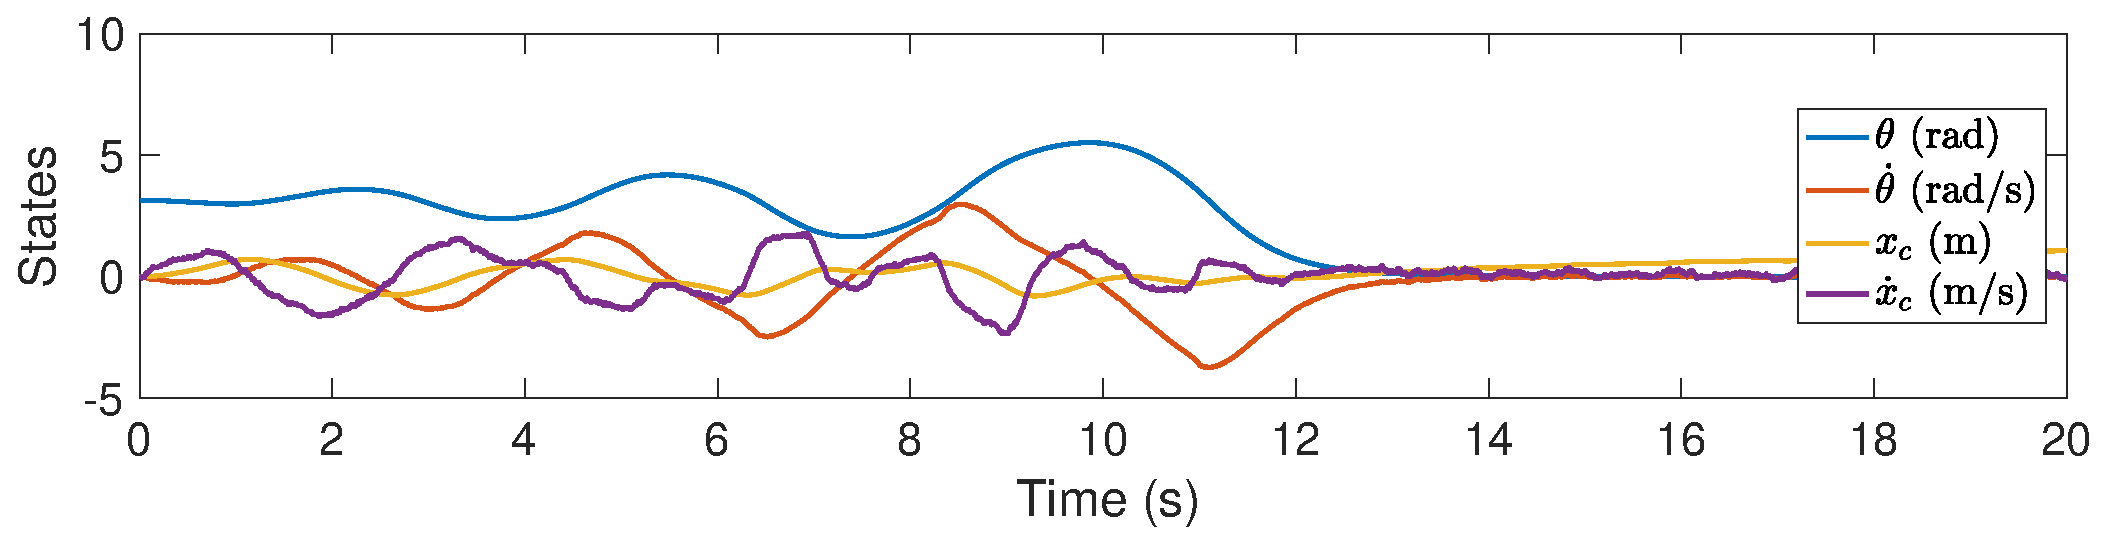
\includegraphics[width=1\columnwidth, keepaspectratio]{MC_states_1.eps}
    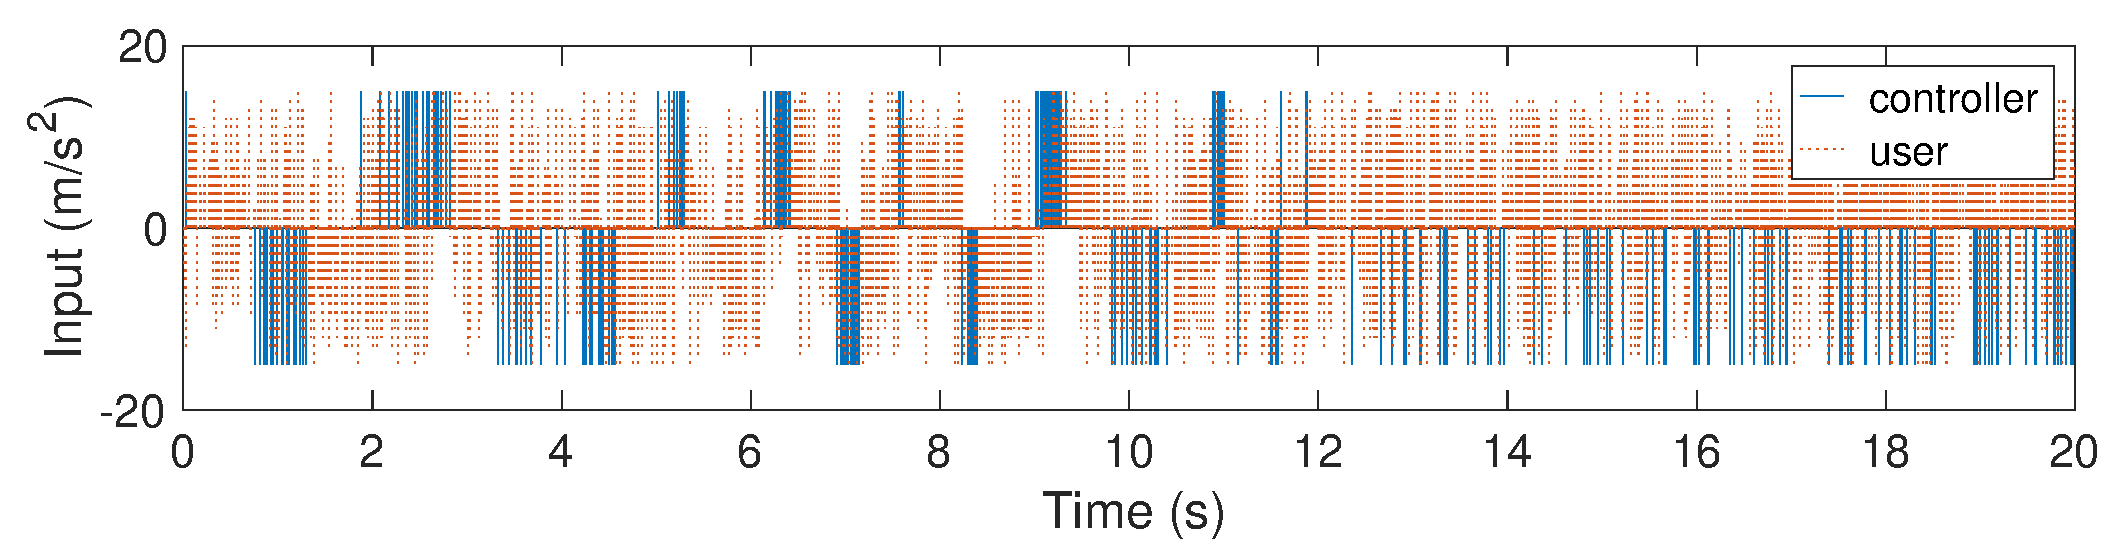
\includegraphics[width=1\columnwidth, keepaspectratio]{MC_control_1.eps}
    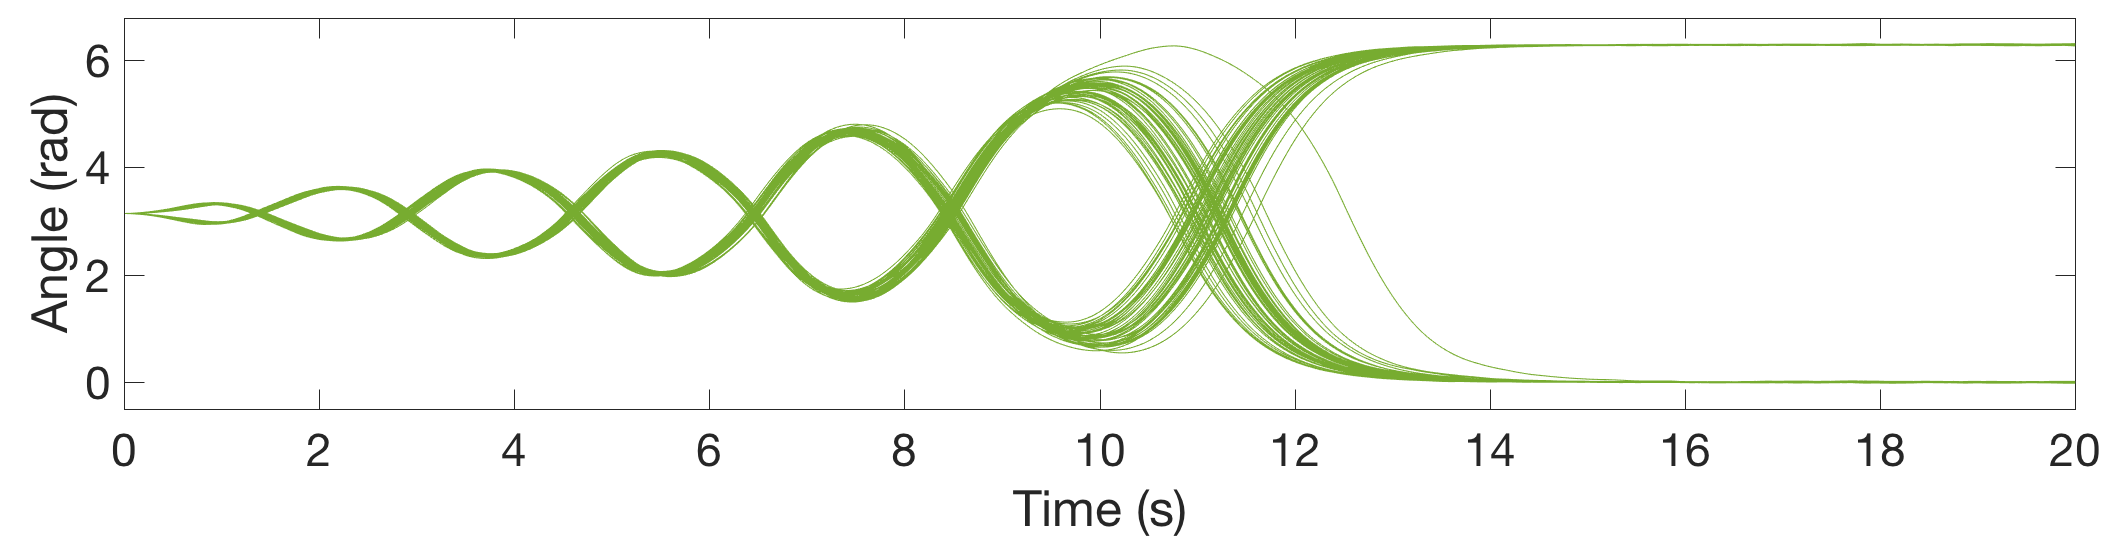
\includegraphics[width=1\columnwidth, keepaspectratio]{MC_angle_100.eps}
\end{center}
\caption{For the cart pendulum inversion task, noise input with a MIG-based filter in assistance mode is able to invert the pendulum in 100 out of 100 of the simulation ran. (top, middle) An example trial with the system evolution and filtered input are shown. (bottom) Convergence results from all 100 trials.}
\label{fig: MC_cp}
\end{figure}

A series of 100 Monte Carlo simulations were run for unskilled users (as modeled using Gaussian noise) attempting the task of cart pendulum inversion. System behavior, simulated user input, and controller intervention during an example trial are visible in Fig.~\ref{fig: MC_cp}. Results of the 100 trials with noise input demonstrate a $100\%$ success rate and are also shown in the figure.

What is more, we are interested in how controller intervention changes according to the skill level of a user. We note close to $0\%$ intervention for a simulated skilled user and $\sim50\%$ intervention for noise input, which makes sense in this one-dimension-controlled task of inverting a pendulum. 

Note that for simulated users the relationship between skill and controller intervention is explicit ($0\%$ intervention for an always successful user and $\sim50\%$ for noise input). With human subjects, such a relationship is more difficult to assess, because we can only approximate users' skill level and cannot account for momentary mistakes. However, we perform an analysis on data collected in a human subject experiment described in Chapter~\ref{chapter: training}. We identify a weak but analogous relationship between subjects' estimated skill level and controller engagement when using the MIG-based filter in training mode. 


\section{Safety-Oriented Assistance}

Next, we analyze the performance of MIG-based assistance on a spring-loaded inverted pendulum (SLIP) model. For our experiments, we use simulated users modeled using MPCs with differing objective functions as described in Section~\ref{section: simulated users} of Chapter~\ref{chapter: methods}. 

We show that with the MIG filter in assistance mode the SLIP can be kept upright even when input is provided by Gaussian noise or a low-skill user. From Fig.~\ref{fig: SLIP_noise} we see that for noise input the filter allows the foot to make random movements and the SLIP to change direction, while keeping the center of mass oscillating around a safe constant height. 


\begin{figure}[!t]
\begin{center}
   	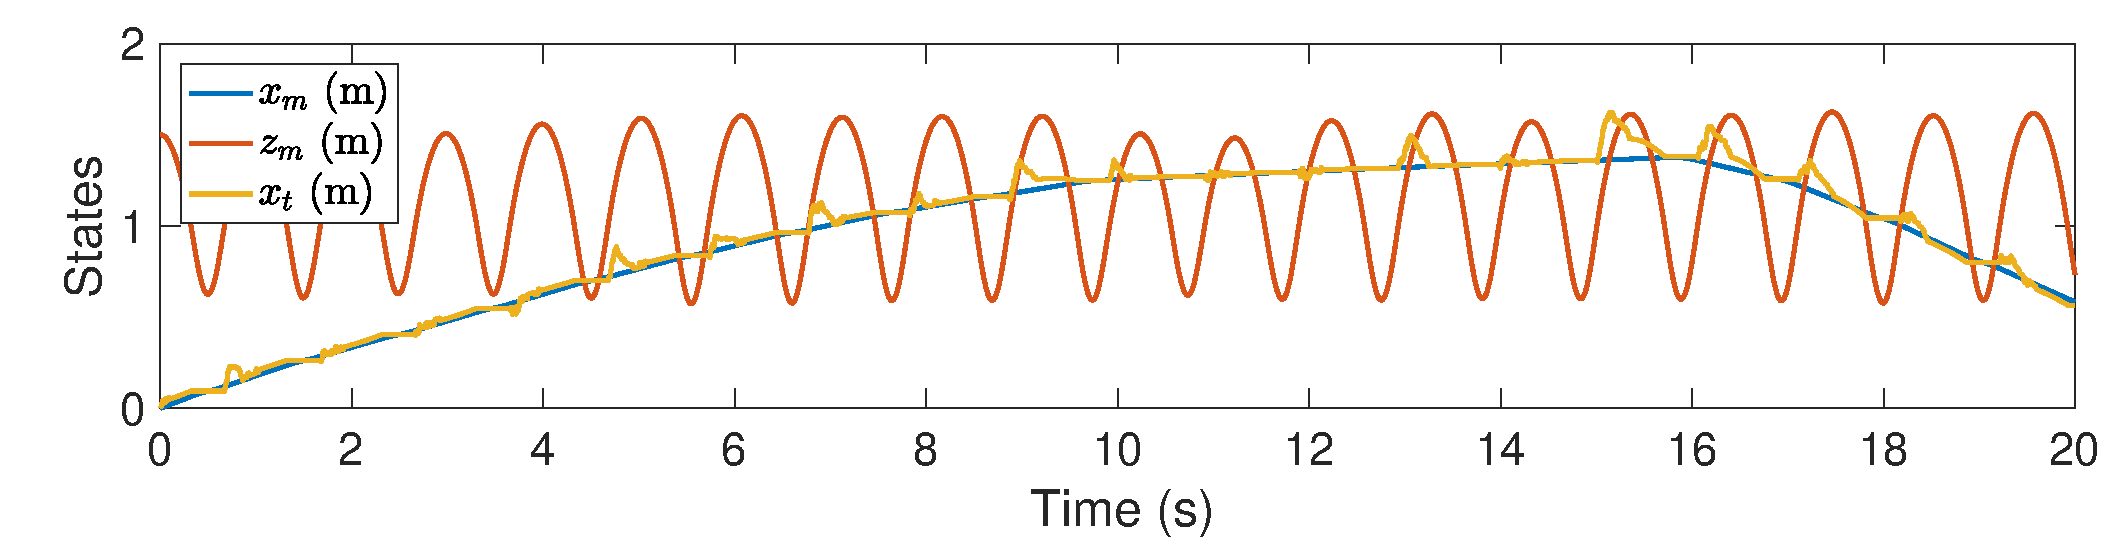
\includegraphics[width=1\columnwidth, keepaspectratio]{SLIP_noise_states.eps}
\end{center}
\caption{We simulate a SLIP model using Gaussian noise as user input and the MIG-filter in assistance mode for support. Note that the filter allows the foot to make random movements and the SLIP to change direction, while keeping the center of mass oscillating around a safe constant height. The controller overrides the user's input for $\sim70\%$ of the simulation time.}

\label{fig: SLIP_noise}
\end{figure}
\begin{figure}[!t]
\begin{center}
  	\includegraphics[width=1\columnwidth, keepaspectratio]{SLIP1_noassist_velocity.eps}
  	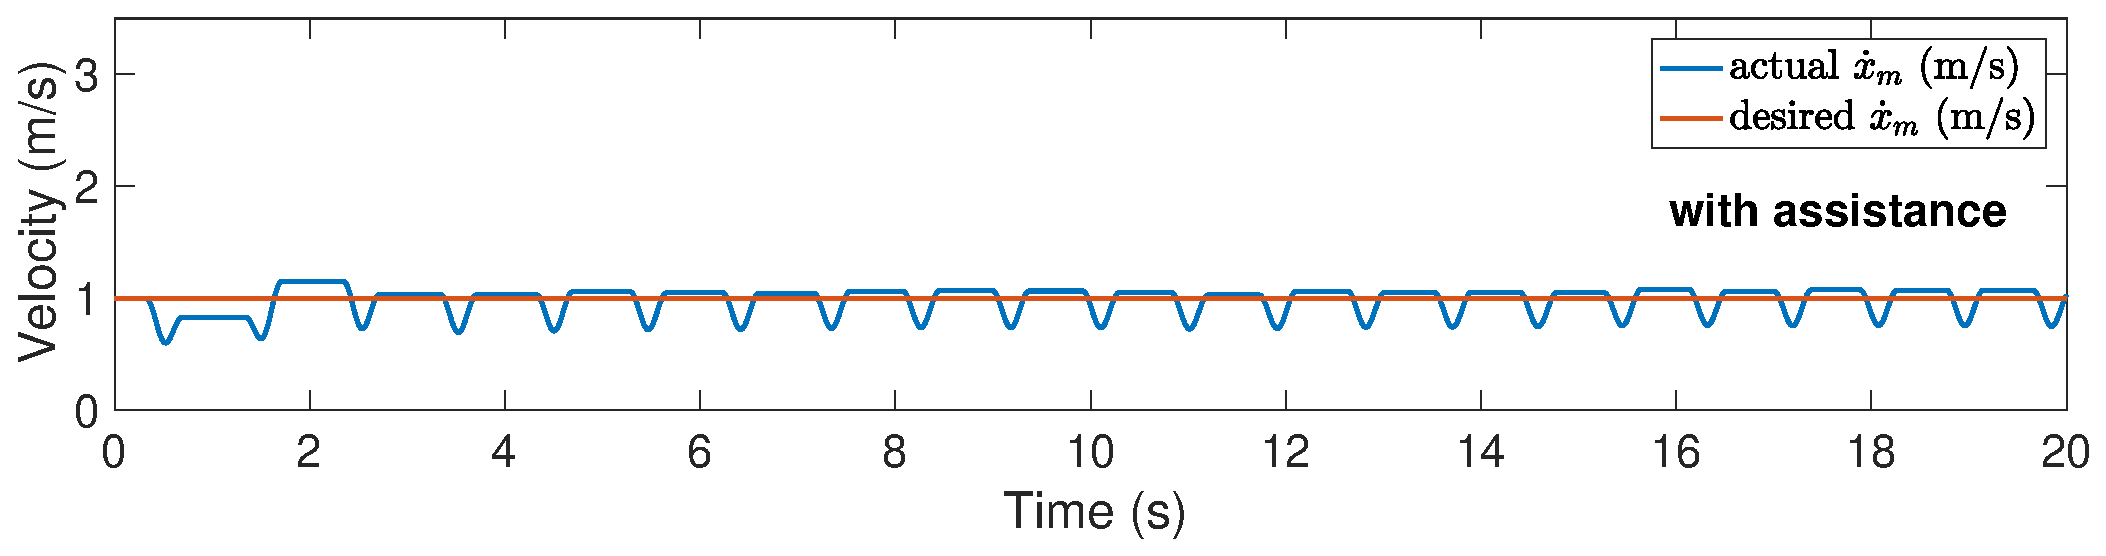
\includegraphics[width=1\columnwidth, keepaspectratio]{SLIP1_assist_velocity.eps}
\end{center}
\caption{(top) We simulate a low-skill user that attempts to move forward with no assistance. The SLIP falls after $\sim5.5s$. (bottom) We use the same user simulation but now the controller helps the user keep balance without restricting its forward motion. With under $40\%$ controller intervention, the SLIP establishes a cyclic gait and maintains an average speed of $0.98~m/s$ (close to the user's desired $1~m/s$).}
\label{fig: SLIP_weak}
\end{figure}

\begin{figure}[!t]
\begin{center}
   	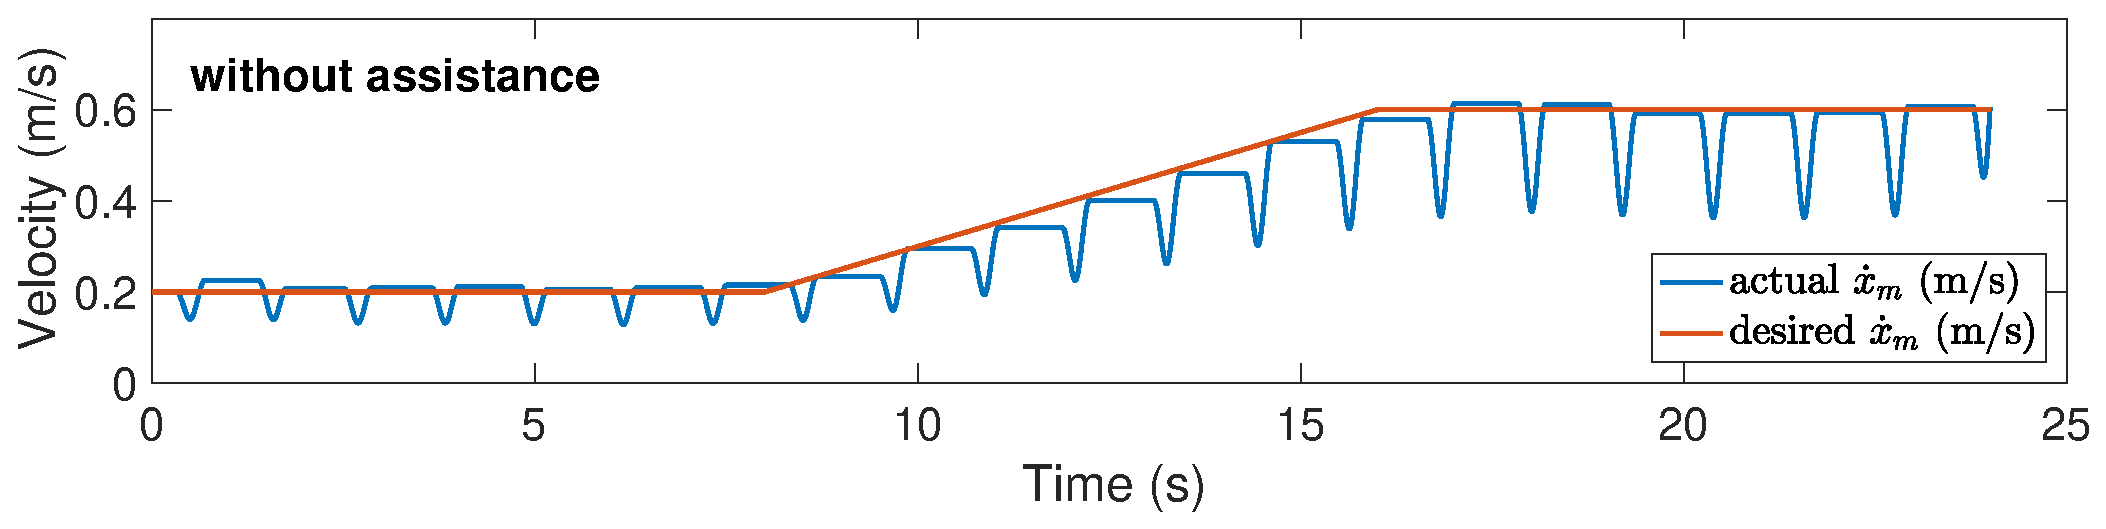
\includegraphics[width=1\columnwidth, keepaspectratio]{SLIP2_noassist_velocity.eps}
   	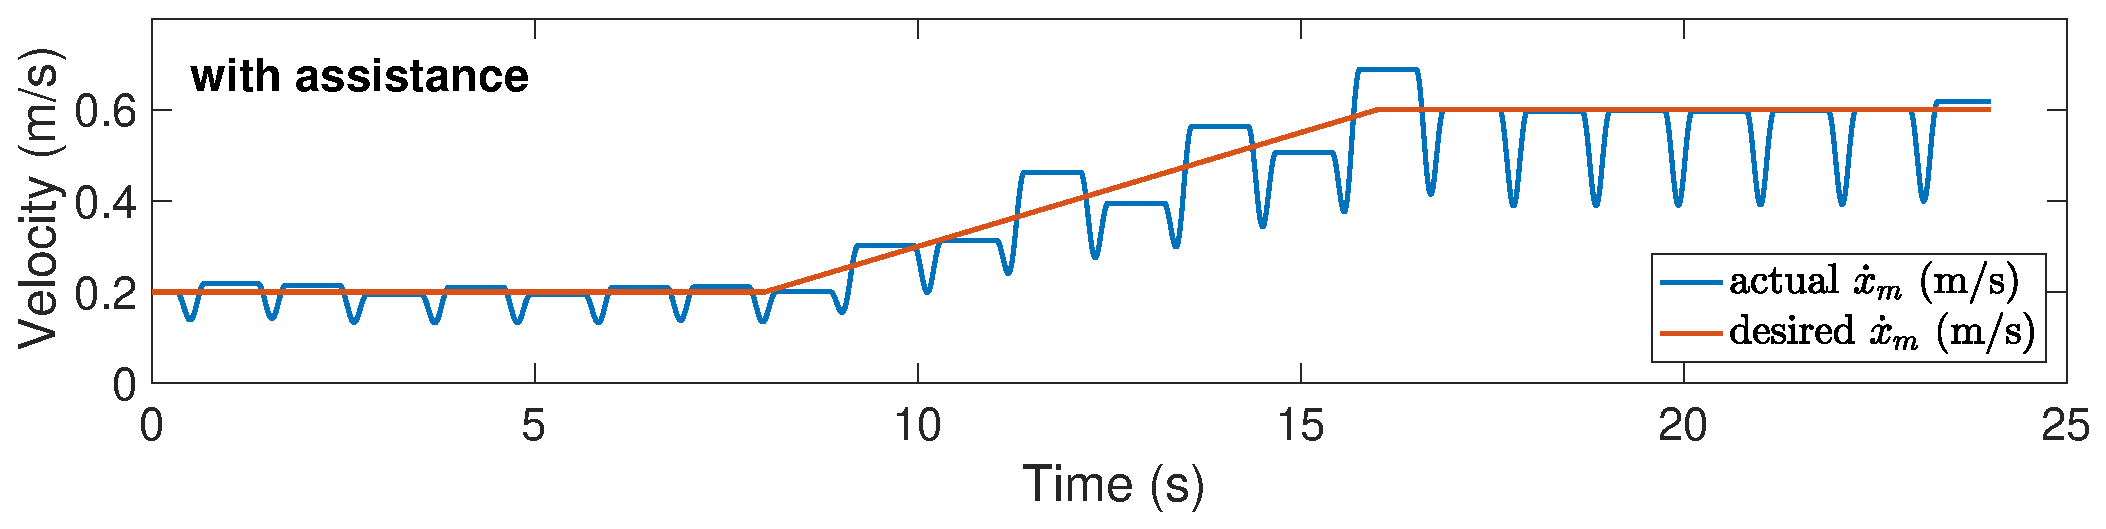
\includegraphics[width=1\columnwidth, keepaspectratio]{SLIP2_assist_velocity.eps}
\end{center}
\caption{(top) We simulate a capable user that attempts to move forward with varying velocity. (bottom) We simulate the same user with added assistance. Note that the assistance does not impede the user's forward motion, even though the controller has no \textit{a priori} knowledge of the user's desired velocity. The controller intervenes $\sim~20\%$ of the time.}
\label{fig: SLIP_skilled}
\end{figure}

For a low-skill user, the assistance prevents the SLIP from falling, while allowing it to maintain its desired forward velocity, as visible in Fig.~\ref{fig: SLIP_weak}. Finally, when provided with input from a skilled user, the filter allows the user to dictate its desired forward velocity and interferes only minimally with its desired motion, as visible in Fig.~\ref{fig: SLIP_skilled}. 

What is worth noting is that the controller overrides user input for $\sim70\%$ of the time for noise input, for under $40\%$ of the time for a low-skill user, and for $\sim~20\%$ of the time for a skilled user. Again, we see a relationship between the skill of the user and controller engagement. The more skilled a user is at the task, the less the controller interferes, while even for noise input the controller is able to keep the hopper upright and safe. 

Based on these results, the MIG criterion shows promise to be used in assistance-oriented applications, such as lower-limb exoskeletons \cite{exoskeletons}. In walking assistance, we want to at all cost prevent users from falling, while at the same time giving them freedom to follow their natural gait pattern, walk at a desired pace, and change speeds or stop when convenient. Such an implementation of the shared control paradigm will be evaluated in future work. 

